\section{Computer Experiments} \label{ch:computer_experiments}
This section describes the setup and configuration of the computational experiments conducted in this study, and the accompanied results. Two types of statistical models, \acrshort{convlstm} and \acrshort{ar}-model are trained and evaluated on a unseen portion of the dataset. 

\subsection{Hardware} \label{sec:hardware}
%How to deal with big datasets that will easily eat up you memory? ``Big data'' involve processing large amounts of data that does not fit into memory. Processing substantial amounts of data require expert knowledge about distributed systems and analysing for system bottlenecks.  %Although theoretically fascinating it remains to see if \acrshort{convlstm} provide a clear practical advantage over the autoregressive models.
%Conducting experiments on big datasets require external computational resources.  
The experiments described below, is conducted on a 
%This study had access to a 
DGX-2 system consisting of 16 NVIDIA Tesla V100 GPUs, each of 32Gb local memory and 1.5Tb shared memory. %The resources was available through the \acrfull{ex3} project hosted at Simula. 
This study was awarded access 1 GPU and 1024G part of the memory. The data is stored on a \acrfull{rdma} accessed over Infiniband. \textit{The best choice of collective implementation depends upon the number and kind of GPUs, and the network interconnect in the cluster.} The DGX-2 system is designed for a high level concurrency and scheduling workers competing for system resources.
%The hardware sets the limitations for efficiency of pipelines and training procedure. 
%\textit{NVIDIA V100 GPU -- The eX3 infrastructure includes a DGX-2 system consisting of 16 NVIDIA Tesla V100 GPUs, allowing simultaneous communication between all eight GPU pairs at 300 GBps through the 12 integrated NVSwitches. This gives a theoretical system-wide system bi-directional  bandwidth of 2.4 TBps. All GPUs have 32 GB of local memory (total of 512 GB) and share a 1.5 TB main memory. The total system has 81,920 CUDA cores, and 10,240 Tensor cores delivering 2 Petaflops of tensor performance. The peak performance in double precision is 125 Teraflops.}
%Working on such a monstrosity pose additional challenges related to porting existing code and virtual environments, developing and debugging code. To eventually end up with an%a achieved 
%acceptable level of efficiency and reliability. \textbf{må de siteres? (\cite{ex3docs} and \cite{ex3homepage}).} 
\begin{table}[ht]
    \centering
    \begin{tabular}{c|c}
        Device &  Type  \\ \hline
        GPU & Tesla V100-SXM3-32GB \\
        CPU & DualProcessor AMD Epyc7601 (SMT2) w/2TB ram and 4TB NVMe 
    \end{tabular}
    \caption{Hardware specifications for the environment used on \acrshort{ex3}. Operating system is Ubuntu 18.04.4.}
    \label{tab:hardware_ex3}
\end{table}

\subsection{Framework} \label{sec:framework}
%\textbf{Make sure this section contains what you intend to say about the software.}
Details regarded project repository and virtual environments is available in Section \ref{sec:structure_and_implementations}. This section describes the implementation and compilation of the models.

The \acrshort{convlstm} is implemented using Tensorflow's keras API which simplifies many aspects of building and executing machine learning models. Its implementation and distribution system aware, making the code more versatile. %Easily portable between systems.
The \acrshort{ar}-models are trained and evaluated using self implemented modules. The idea was to utilize the analytical solution of the least squares problem. Many regression modules provide a numerical solution, not the analytical. The python package ``sciclouds'' provide a self implemented version of \acrshort{ar}-models, using the analytical solution to the least squares problem derived in Section \ref{sec:ARmodels}.

%Complex computations will cause memory growth, dependant on how many intermediate computations it needs to store. This is the case for \acrshort{convlstm}. To speed up the development process the software is developed on a subset of \acrshort{ecc}. Small adjustments needs to be made, running experiments on the entire data. For instance threads deadlock when extracting large amounts of data. This is a precautionary measure to avoid overloading the system. \textbf{Possible to develop code to do Hyperparameter tuning based on }
%For a more detailed description please see the project repository described in Section \ref{sec:structure_and_implementations}.

\subsection{Model Setup and Evaluation}
The following sections contain the configurations of the models compiled for this study along with descriptions of hyperparameters. A hyperparameter is a parameter set before the training starts, as mentioned in Section \textbf{ref somewhere in numerical methods}. A model is compiled based on a choice of hyperparameters. In the search for the best model configuration, different combinations of hyperparameters are tested. This is done manually to begin with since the choice of architecture can easily overload the system memory resources.
 
As a starting point for the \acrshort{convlstm} is the set of architectures provided by \citeauthor{SunAirLSTM} (\citeyear{SunAirLSTM}) described in Section \ref{sec:related_work}. For the \acrshort{ar}-models it follows the principal of starting with the simplest model possible and increasing the complexity from there. 
%Stopping at architectures where increased complexity don't increase the performance? Know stategies are using spaced sampling, attempting lags of 1, 2, 5, 10. The second is naturally to further investigate regons of lags showing the most promise. 
%on a similar problem, air quality forecasting problem was executed. \citepaper{chollet2015kerastuner} provide suitable software for the automatic hyperparameter tuning. 
%\textbf{Man kjører eksperimenter på mange modeller ved å bruke traning og validations dataset. The choice of model is based on this data basis and then it performance is tested on the test dataset.} 

The partitioning into training and test data is inherited from the model. Since the AR-modelling is done based on a analytical solution there is no need for a validation dataset. Both model are tested on 2014 to 2018. For \acrshort{ar}-models this is trained on 2004 to 2013 and the \acrshort{convlstm} trained on  2004 to 2011 and validated on  2012 to 2013. The test period was chosen based on the assumption that the latest period is most representable for the climate in the near future. Another minor differences for the datasets prepared for the \acrshort{ar} and the \acrshort{convlstm}-models. The order of the \acrshort{ar}-model determine the length of the training sequence. All samples with gaps in the requested sequence is disregarded causing a reduction in the data basis for a model of a particular order, determined by the number of lags. For the \acrshort{convlstm} these gaps are filled with a out-of-sample value, $c=1.5$. 
\begin{enumerate}
    \item \textbf{TODO: check if it predicts out of sample valeus if not try and delete samples if it does delete the samples and retrain best model.}
\end{enumerate}

\subsubsection{Autoregressive models (AR)}
The set of hyperparameters available for ar models are ....
%A set of models are compiled by varying components such as
stadard scaling the predictors, transforming the target, the inclusion of intercept, order of the models and environmental variables. Varying combinations of theses hyperparameters results in the set of models used in this part of the experiments. 
A summary of the calibrated models are provided in Table \ref{tab:ar_model_config}. Keep in mind that one AR-model is the combination of 13041 individual regression models.  

%Time consuming task because of the high number of matrix inversions. A double for loop over this takes to long and \textbf{mention the version of paralelization used on this problem}.

\subsubsection{Feature Scaling} \label{sec:scaling_predictors}
%Feature standardization makes the values of each feature in the data have zero-mean 
Feature scaling is used to standardise the predictor variables.
%By subtraecting the mean and dividing by the variance, t
Applying Equation \ref{eq:scaling_data} to the predictors reshapes the distribution toward a standard normal distribution with zero mean and unit variance. 
%Data transformation can be beneficially in an attempt 
The transformation offers an additional benefit of increased numerical stability. %When applied the predictors is transformed according to the following Equation \ref{eq:scaling_data}. 
The feature scaling is applied after the partition into training and test dataset, the mean and standard deviation is computed based on the training set. In this manner the trained model avoids sneak peaking at the test data, resulting in a unrepresentative measure on performance.
\begin{equation} \label{eq:scaling_data}
    \mathbf{x} = \frac{\mathbf{x} - \bar{\mathbf{x}}}{\sigma_{\mathbf{x}}}
\end{equation}
where $\bar{\mathbf{x}}$ is the average and $\sigma$ is the standard deviation. The model is trained to find relations in transformed data. Before making predictions based on test data it need to be transformed, using the mean and standard deviation from the training sample.

\subsubsection{Transforming target} \label{sec:transforming_target}
A trick to avoid prediction unphysical values is fitting against a transformed target. In this study, the target, \acrfull{cfc} ranges from 0 to 1. By applying the inverse sigmoid transformation, see Equation \ref{eq:sigmoid} \textbf{update to inverse sigmoid} the target takes values from the entire real axis $(-\infty, \infty)$. 
The inverse transformation, ordinary sigmoid, transforms the values back to the range [0, 1]. Thereby alleviating predictions of out-of-sample values. The sigmoid function is shown in figure \ref{fig:activation_func_plus}. 
\begin{figure}
    \centering
    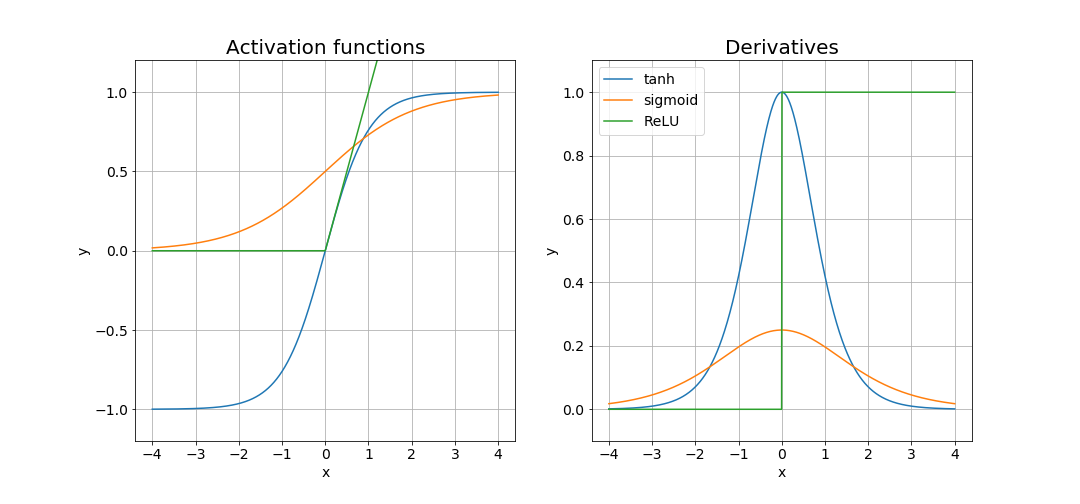
\includegraphics[scale=0.45]{Chapter3_Method/figs/activation_functions_and_derivatives.png}
    \caption{Sigmoid function and other activation functions. \textbf{remove?}}
    \label{fig:activation_func_plus}
\end{figure}

\subsubsection{Lags and Environmental variables}
The dataset for a particular model is a combination of the the number of lags (order of model) and environmental variables such as $t2m$, $sp$, $q$ and $r$ is included. The environmental variables never appear in isolation.
Order the number of time steps of previous cloud cover includes as predictors. All model is trained either on the full set of environmental variables or none of them. No partical inclusion of enviornmental variables. \textbf{Check magnitude of weights and determine/discuss whether any of them can be excluded.}

\subsubsection{Experimental setup (AR-models)}
Table \ref{tab:ar_model_config} shows a summary of the \acrshort{ar}-models included in this study. The naming conventions used $AR_{STB_L}$ or $TR_{STB_L}$. B stands for bias, T for scaling predictors, S for sigmoid transformation of the target and L for the number of lags, previos timestep of cloud cover included. AR og Tr describe whether the enviormental variables are included in the dataset of not. This descrition elaborated in Table \ref{tab:ar_model_config}. Bias and Transformation is mutually exclusive, it doesn't make sense to add bias when transforming the predictores.

\begin{table}[h]
    \centering
    \resizebox{\textwidth}{!}{%
    \begin{tabular}{cccccc}
    \cline{2-5}
     & \textbf{Scaling predictors} & \textbf{Transforming target} & \textbf{Lag} & \textbf{Environmental variables} & \textbf{Bias}\\ \hline
    \multicolumn{1}{c}{\textbf{$TR_{SB_1}$}} & \checked & $\times$  & 1 & $\times$ & \checked   \\ \hline
    \multicolumn{1}{c}{\textbf{$AR_{SB_0}$}} & \checked & $\times$  & 0 & \checked  & \checked  \\ \hline
    \multicolumn{1}{c}{\textbf{$AR_{SB_1}$}} & \checked & $\times$  & 1 & \checked & \checked  \\ \hline
    \multicolumn{1}{c}{\textbf{$AR_{SB_2}$}} & \checked & $\times$  & 2 & \checked & \checked  \\ \hline
    \multicolumn{1}{c}{\textbf{$AR_{SB_3}$}} & \checked & $\times$  & 3 & \checked & \checked  \\ \hline
    \multicolumn{1}{c}{\textbf{$AR_{SB_4}$}} & \checked & $\times$  & 4 & \checked & \checked  \\ \hline
    \end{tabular}%
    }
    \caption{Configuration of \acrshort{ar}-models. $\times$ denoted not applied, \checked denotes applied. \textbf{Bruk denne for tre eksempler.}}
    \label{tab:ar_model_config}
\end{table}

\begin{figure}
    \centering
    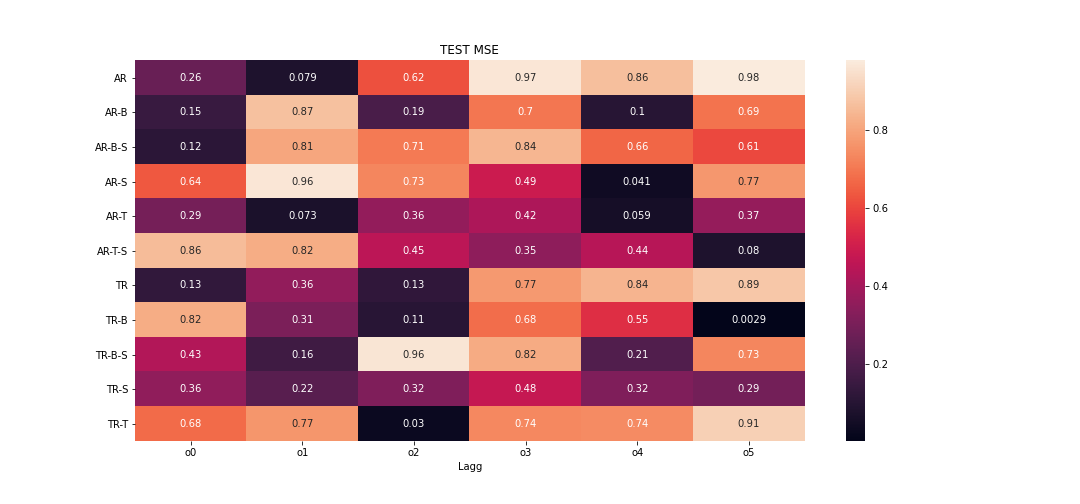
\includegraphics[scale = 0.5]{python_figs/MSE_score_AR_models.png}
    \caption{MSE score for a set of configured AR models}
    \label{fig:results_ar_models}
\end{figure}

\subsection{Convolutional LSTM (ConvLSTM)}

The formulation of the Air quality forecasting problem presented by  \citeauthor{SunAirLSTM} is similar to the formulation of the cloud fractional cover prediction problem presented in this project. The machine learning experimental setup is adopted from the paper \citepaper{SunAirLSTM}. 
% Endrer på arkitekturen - denne bruker -train - validation - test, en hvis prosentandel a
A lot of architectural decisions (batch size, sequence length, number filterers and number layer) can cause the \acrshort{gpu} to run out of memory. In these cases the compiled model is not trainable. Between each layer is a layer of Batch Normalization. According to the paper \citepaper{ioffe2015batch} this shold simplify the trainingprocess. The feature was added between each layer. Epochs is the number of times the model has seen the entire dataset. The dataset is partitioned into subsets called batches. The batch size is the number of samples a weight update is based on. The sequence length is the \textbf{quite selv explanatory, still need to explain it.. } Number of hidden states .. 

\subsubsection{Experimental setup (ConvLSTM)}
Models are given names based on a extension of the convention from \citepaper{SunAirLSTM}. The paper introduce the convention ConvLSTM-hidden states-filter$\times$filter. Adding the batch size and sequence length as variables, it becomes $ConvLSTM-B_{x}-SL_{y}-hidden states-filter$\times$filter$

\begin{table}[]
    \centering
    \resizebox{\textwidth}{!}{%
    \begin{tabular}{cccccc}
     & \textbf{Sequence Length} & \textbf{Batch Size} & \textbf{Hidden States} & \textbf{Kernels} & \textbf{Num. Parameters} \\ \hline
    \textbf{$ConvLSTM-B_{5}-SL_{24}-256-3\times3-256-3\times3$} & 24 & 5 & [256, 256]   & [3, 3] & 98347984 \\ \hline
    \textbf{$ConvLSTM-B_{15}-SL_{24}-256-5\times5-256-5\times5$} & 24 & 15 & [256, 256]  & [5, 5] & 4244308 \\ \hline
    \textbf{$ConvLSTM-B_{10}-SL_{24}-128-1\times1-128-1\times1$} & 24 & 10 &  [128, 128] & [1, 1] & 0927502 \\ \hline
    \textbf{$ConvLSTM-B_{5}-SL_{6}-64-3\times3-64-3\times3$} & 6 & 5 & [64, 64]      & [3, 3] & 9472 \\ \hline
    \textbf{$ConvLSTM-B_{5}-SL_{6}-256-3\times3-256-3\times3$} & 6 & 5 & [64, 32]      & [3, 3] & 380495 \\ \hline
    \textbf{$ConvLSTM-B_{5}-SL_{6}-8-3\times3-8-3\times3-8-3\times3$} & 6 & 5 & [8, 8, 8]     & [3, 3, 3] &  20934802\\ \hline
    \end{tabular}%
    }
    \caption{Give three examples to simplify the explanation of configurations and models.}
    \label{tab:convlstm_config}
\end{table}

\begin{enumerate}
    \item \textbf{TODO: Add drawing of best convolutional lstm model from tikz! Simplyfies the explenation.}
    \item \textbf{TODO: Add heatmap of model results, Evaluated on TEST data so its the same as the AR results. To make a heatmap its natural to vary to components Maybee models config and sequence length?}
    \item \textbf{TODO: Show loss curve for the best model.}
\end{enumerate}



\subsection{Results on Predicting sequence}
The foundation of the choice of the best model is different for \acrshort{ar} and \acrshort{convlstm}-models. As mentioned in Chapter \ref{ch:num_methods}, the \acrshort{ar}-model is optimized to fit the next timestep, while the \acrshort{convlstm} is trained to fit a sequence or a predescribed length. In this section the best ar model and convlstm model are assed on how well they predict the sequence length og the best convlstm model. By feeding the prediction into the ar model, one can modify its ability to predict sequences. The two best models are X and Y, with performance measured by the MAE metric of A and respectively. 

%\subsubsection{Visual Comparison predicting a sequence of length}
Visualizing the experiments 
%%%% TARGET PREDICITON ERA5
\begin{figure}[ht]
    \centering
    \includegraphics{python_figs/target_prediction_era5_plot_horizonal.pdf}
    \caption{\textbf{Update to AR, ConvLSTM, target - the number of rows is the sequence length} Comparison target, predicted and era5 horizontal cloud fractional cover. Imagine this plot, with a row for each step in the predicted sequence and each column being (AR, Convlstm, target)}
    \label{fig:target_predict_era5_horizontal}
\end{figure}

Some text where you comment the results from this comparison. Is it evident that the convLSTM is better at predicting spatial patterens as expected or does it all resemble random noise. Is the predicted values in sample or out of sample.

If the results are bad, the conclusion is that the dataset is not of high enough quality. This is not uncommon when working with cloud data. Don't make it look like you took bad choises when building the dataset it may simply mean that the nature of the problem is difficult. Which it is..


\subsection{Other figures}
%%%% TARGET PREDICITON ERA5
\begin{figure}[ht]
    \centering
    \includegraphics{python_figs/target_prediction_era5_plot_horizonal.pdf}
    \caption{Comparison target, predicted and era5 horizontal cloud fractional cover. Imagine this plot, with a row for each step in the predicted sequence and each column being (AR, Convlstm, target)}
    \label{fig:target_predict_era5_horizontal}
\end{figure}

%\subsection{Autoregressive models}
%%%% TARGET PREDICITON HORIZONTAL
\begin{figure}[ht]
    \centering
    \includegraphics{python_figs/target_prediction_plot_horizonal.pdf}
    \caption{Comparison target and predicted cloud fractional cover.}
    \label{fig:target_predict_horizontal}
\end{figure}

%%%% TARGET PREDICITON HORIZONTAL
\begin{figure}[ht]
    \centering
    \includegraphics{python_figs/target_prediction_plot_vertical.pdf}
    \caption{Comparison target and predicted vertical cloud fractional cover.}
    \label{fig:target_predict_vertical}
\end{figure}

\section{Practical implications - OUTDATED} \label{sec:practical_implications}
It is necessary to have a understanding of the needs of the end product before conducting large machine learning projects. Answering questions like: What will it be used for and how can it be implemented in useful way?

A major downside of the data driven learning approach is the rigid resolution. A trained model can only be used on similar problems, with the same spatiotemporal resolution. For applications like climate models, output comes in a wide range of different resolutions. Before implementing the finished product in a new model of a different resolution, it would need to be retrained on the resolution of the climate model under development. This process involves both remapping of the dataset and retraining the model at the correct resolution. This is a time consuming process involving finding a new set of hyperparameters suitable for the new resolution. % It essentially means starting over.

Once trained on global climate datasets, machine learning models provide fast results even for complex parameterization which is what makes them suitable for the application of climate modelling. Most machine learning packages are developed using Python. \acrfull{esm} are implemented in python. Methods for including the trained parameterizations need to be developed.
 
\subsection{Any implications based on the results presented in this chapter.}